\documentclass[a4paper, 11pt]{article}

\usepackage[utf8x]{inputenc}
\usepackage[T1]{fontenc}
\usepackage{ucs}
\usepackage[english]{babel}
\usepackage{mathtools}
\usepackage{amsmath}
\usepackage{amsfonts}
\usepackage{ulem}
\usepackage{verbatim}
\usepackage{fancyhdr}
\usepackage[parfill]{parskip}
\usepackage{graphicx}
\usepackage{palatino}
\usepackage{float}
\usepackage[font={small,it}]{caption}

\linespread{1.05}
\pagestyle{fancyplain}
\fancyhead{}
\fancyfoot[L]{}
\fancyfoot[C]{}
\fancyfoot[R]{\thepage}
\renewcommand{\headrulewidth}{0pt}
\renewcommand{\footrulewidth}{0pt}
\setlength{\headheight}{13.6pt}

\widowpenalty=1000
\clubpenalty=1000

\newcommand{\horrule}[1]{\rule{\linewidth}{#1}}

\title{ 
\normalfont \normalsize 
\textsc{University of Copenhagen} \\ [25pt]
\horrule{0.5pt} \\[0.4cm]
\huge PCSD: Assignment 2 \\
\horrule{2pt} \\[0.5cm]
}

\author{Jens Fredskov (chw752)\\Henrik Bendt (gwk553)\\Ronni Lindsgaard (mxb392)} % Your name

\date{\normalsize\today} % Today's date or a custom date

\begin{document}
\maketitle
\pagebreak

\section{Serializability \& Locking} % (fold)
\label{sec:serializability_&_locking}

The predecence graph for Schedule 1 can be seen in figure \ref{fig:schedule1}.
As there is a cycle the schedule is not conflict-serializable. The schedule
could not have been generated using strict two-phase locking as the write to X
in T2 needs to happen after the read in T1. T1 cannot be completed and thus
releasing the lock of X as T3 needs to release the read lock for Y. T3 cannot
run before T2 which is visible in the predence graph. 

\begin{figure}[H]
  \centering
  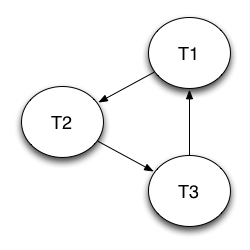
\includegraphics[width=0.5\textwidth]{images/schedule1}
  \caption{Precedence graph for Schedule 1. The cycle shows that the schedule is
  not conflict-serializable.}
  \label{fig:schedule1}
\end{figure}


Figure \ref{fig:schedule2} show the precedence graph for Schedule 2. There is no
cycle which means it is conflict serializable. Figure \ref{fig:schedule2-2pl}
shows injected read/write locks in accordance with strict 2PL rules.
 
\begin{figure}[H]
  \centering
  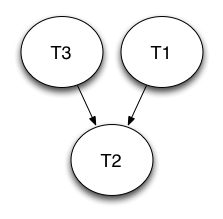
\includegraphics[width=0.5\textwidth]{images/schedule2}
  \footnotesize
  \caption{Precedence graph for Schedule 2. The absence of a cycle show that the
  schedule is conflict-serializable.}
  \label{fig:schedule2}
\end{figure}

\begin{figure}[H]
\footnotesize
\centering
\verbatiminput{figures/schedule2-2pl.txt}
\caption{Schedule 2 with read- (RL) and writelocks (WL) induced. All locks are
released on commits. The unlock operations are omitted for simplicity of the
table.}
\label{fig:schedule2-2pl}
\end{figure}


% section serializability_&_locking (end)

\section{Optimistic Concurrency Control} % (fold)
\label{sec:optimistic_concurrency_control}

\paragraph{Scenario 1} % (fold)
\label{par:scenario_1}

Here test 2 applies, but as the intersection of the write set for T2 and the read set for T3 equals $\{4\}$, T3 is not allowed to commit and must roll back.

% paragraph scenario_1 (end)

\paragraph{Scenario 2} % (fold)
\label{par:scenario_2}

Here test 2 applies, but as the intersection of the write set for T1 and the read set for T3 equals $\{3\}$, T3 is not allowed to commit and must roll back. 

% paragraph scenario_2 (end)

\paragraph{Scenario 3} % (fold)
\label{par:scenario_3}

Here test 2 applies both between T1/T3 and T2/T3. As both tests pass T3 is allowed to commit.

% paragraph scenario_3 (end)

% section optimistic_concurrency_control (end)

\pagebreak
\section{Questions for Discussion on the Concurrent Implementation of Bookstore} % (fold)
\label{sec:questions_for_discussion_on_the_concurrent_implementation_of_bookstore}

\paragraph{1.} % (fold)
\label{par:1_}

The locking protocol should be correct. Our reasons for believing this are as follows: First of all of our tests pass, which (depending of the tests) is an indicator of correctness.

Regarding predicate reads these could occur with respect to ISBN or editor pick. When we get editor picks we get a shared lock on the entire map, meaning that these are protected. As we have no function to get a single ISBN we always get the entire map and therefore also a shared lock.

More importantly the scheme implemented follows a strict 2PL multi granularity lock. We acquire locks when they are needed, and then let go of all of them at the same time in the end of each function. As the protocol is multi granular it includes both exclusive (write), shared (read), intention exclusive (write further down the hierarchy) and intention shared (read further down the hierarchy) locks.

% paragraph 1_ (end)

\paragraph{2.} % (fold)
\label{par:2_}

The protocol can currently lead to deadlocks, when we try to take locks on individual books (not if we do take read or write locks on the entire map). An example is when two threads try to update two books, where they might try to take the locks of the books in different order and therefore end up in a deadlock.

There are different ways in which we could have gotten around this. A solution could be to sort the books on their ISBN and take the locks in this order, effectively avoiding dead locks. This way of ordering the locks while avoiding dead locks could however lead to a slow down in performance when we need to sort a large number of books before acquiring the locks.

Another possible solution is to lock the entire map in the places where we might risk a dead lock. This solution however is not preferable as it would significantly reduce concurrency.

% paragraph 2_ (end)

\paragraph{3.} % (fold)
\label{par:3_}

There should be no major bottlenecks due to the locking protocol, with respect to the number of clients. One possible bottleneck is when we need to lock down the entire map, as this causes everyone to wait. We however only need to take an exclusive lock on the entire map when adding elements to it, thus we rarely lock down everything. So as long as the client do not try to mainly modify the same books we should not see significant scalability issues stemming for the locks.

% paragraph 3_ (end)

\paragraph{4.} % (fold)
\label{par:4_}

The degree of concurrency we get should greatly exceed the overhead being paid in the locking protocol. Instantiating the locks should not require a significant amount of extra resources, and as the locking protocol is multi granular is allows most threads to work concurrently on books (except for when two thread want two modify the same book, or a thread wishes to modify the entire map).

% paragraph 4_ (end)

% section questions_for_discussion_on_the_concurrent_implementation_of_bookstore (end)

\section{Additional tests} % (fold)
\label{sec:additional_tests}

\paragraph{test3} % (fold)
\label{par:test3}

Tests atomicity. This works by running two threads which concurrently updates copies, and then finally checks whether the final number matches the sum of the two updates plus the original number. The two threads first add books, we then check whether the new number of books match the expected and buys back the same number of books.

% paragraph test3 (end)

\paragraph{test4} % (fold)
\label{par:test4}

Tests that updates are consistent, like test2, but with more threads. One additional thread updates each book of the set, one by one. One additional thread only buys the set of books, while another only replenish it. Thus at each snapshot, the number of books should be a modulus of the number of copies bought/added each time. The end number should be the initial number.

% paragraph test4 (end)

% section additional_tests (end)

\end{document}

